% This file was created with tikzplotlib v0.10.1.
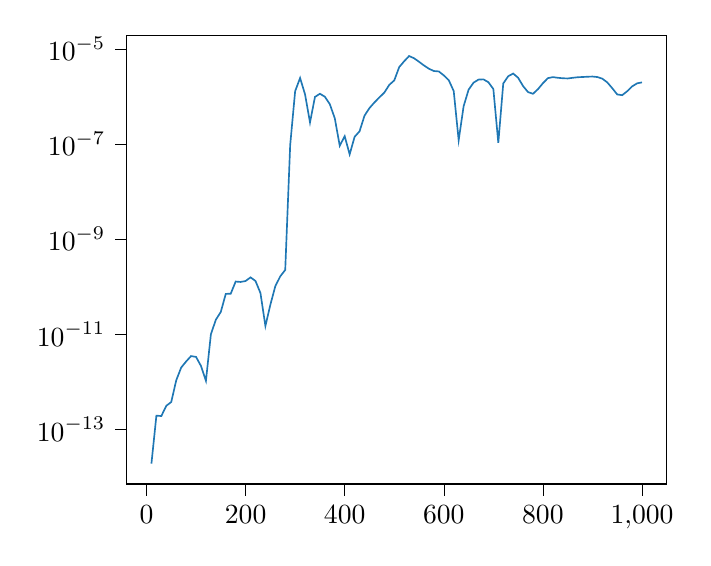
\begin{tikzpicture}

\definecolor{darkgray176}{RGB}{176,176,176}
\definecolor{steelblue31119180}{RGB}{31,119,180}

\begin{axis}[
log basis y={10},
tick align=outside,
tick pos=left,
x grid style={darkgray176},
xmin=-39.5, xmax=1049.5,
xtick style={color=black},
y grid style={darkgray176},
ymin=7.02297163755725e-15, ymax=1.89627393708271e-05,
ymode=log,
ytick style={color=black},
ytick={1e-17,1e-15,1e-13,1e-11,1e-09,1e-07,1e-05,0.001,0.1},
yticklabels={
  \(\displaystyle {10^{-17}}\),
  \(\displaystyle {10^{-15}}\),
  \(\displaystyle {10^{-13}}\),
  \(\displaystyle {10^{-11}}\),
  \(\displaystyle {10^{-9}}\),
  \(\displaystyle {10^{-7}}\),
  \(\displaystyle {10^{-5}}\),
  \(\displaystyle {10^{-3}}\),
  \(\displaystyle {10^{-1}}\)
}
]
\addplot [semithick, steelblue31119180]
table {%
10 1.8846035843012e-14
20 1.91929805382074e-13
30 1.8890444763997e-13
40 3.10002024050959e-13
50 3.72341046883662e-13
60 1.06012421063895e-12
70 1.97253324785152e-12
80 2.65137911625857e-12
90 3.44521633444117e-12
100 3.3102964813736e-12
110 2.13565276574457e-12
120 1.0421108420644e-12
130 9.92900206497893e-12
140 2.00431615748897e-11
150 2.9248881094901e-11
160 7.00414726217957e-11
170 7.06853742205027e-11
180 1.27380633818674e-10
190 1.24787069566423e-10
200 1.30798150088651e-10
210 1.55978674420965e-10
220 1.30877142456853e-10
230 7.29749594086115e-11
240 1.47739875888675e-11
250 4.14403233950367e-11
260 1.01696040477606e-10
270 1.63971419775422e-10
280 2.23636414942163e-10
290 9.47412380214452e-08
300 1.28590346840096e-06
310 2.4378937372449e-06
320 1.10275392209425e-06
330 2.82866542813953e-07
340 9.74277166387871e-07
350 1.13708936141932e-06
360 9.83219959282966e-07
370 6.84552756924361e-07
380 3.4675329523004e-07
390 9.1577665672915e-08
400 1.45429054035362e-07
410 6.02842496200129e-08
420 1.41024335445494e-07
430 1.84336532163543e-07
440 3.93644401727733e-07
450 5.68853043128592e-07
460 7.4574532542282e-07
470 9.52595816602897e-07
480 1.20270315674686e-06
490 1.75004918664956e-06
500 2.16874812257462e-06
510 4.12678936878574e-06
520 5.48146996352805e-06
530 7.06646118478482e-06
540 6.33855583644094e-06
550 5.35479089812385e-06
560 4.47388502558543e-06
570 3.81334759470831e-06
580 3.41786575171199e-06
590 3.34773981337799e-06
600 2.76463567978891e-06
610 2.19385648927983e-06
620 1.29628335301946e-06
630 1.19674679791015e-07
640 6.19907906077022e-07
650 1.38336460167587e-06
660 1.94319442396729e-06
670 2.25647705190402e-06
680 2.28185931829689e-06
690 1.98678592686075e-06
700 1.42780334268927e-06
710 1.05426360495764e-07
720 1.87150906955091e-06
730 2.65854015090577e-06
740 3.0237902780908e-06
750 2.46530814781987e-06
760 1.64605145942798e-06
770 1.23094158748643e-06
780 1.13378964329558e-06
790 1.4191626910437e-06
800 1.89090610686754e-06
810 2.41724393369031e-06
820 2.54660278077579e-06
830 2.46484311730577e-06
840 2.40718645543037e-06
850 2.38412684019917e-06
860 2.46034518035926e-06
870 2.5287460183876e-06
880 2.55767773590931e-06
890 2.59130123834994e-06
900 2.6154623234409e-06
910 2.55203280419281e-06
920 2.35096209244556e-06
930 1.96420220485022e-06
940 1.48286886700322e-06
950 1.09719577602585e-06
960 1.06120498489376e-06
970 1.28183711198965e-06
980 1.62260598392944e-06
990 1.88024049689595e-06
1000 1.9715499918263e-06
};
\end{axis}

\end{tikzpicture}
